\chapter{Architettura}

In questo capitolo verranno descritte le scelte architetturali e implementative che stanno alla base del contributo di questa tesi al progetto IoE. 

Lo scenario legato alla mobilità elettrica veicolare è caratterizzato dalla presenza di diversi domini applicativi, piattaforme e parti interessate i quali necessitano di comunicare in modo unificato e trasparente. A tal fine è stato utilizzato il progetto Smart-M3 (\cite{tullio2011}) che è il cuore della nostra architettura. Appoggiandosi sulle tecnologie tipiche del \emph{Semantic Web} Smart-M3 assicura l'interoperabilità tra gli attori in gioco. 

In particolare vedremo come possono coesistere elementi reali ed elementi simulati e come il passaggio dall'uno all'altro sia assolutamente trasparente a tutti i componenti del sistema grazie all'uso di tecnologie ontology-based.

\section{Smart-M3}

Prima di parlare dei componenti strettamente legati a questo progetto è doveroso fare un introduzione alla tecnologia che fa da collante tra di essi ovvero Smart-M3. Capire come funziona Smart-M3 e quali sono i suoi principi è fondamentale al fine di comprendere a fondo il resto di questo documento.

M3 è un architettura middleware per consentire L'interoperabilità delle informazioni in maniera cross-domain, multi-vendor, multi-device, multi-piattaforma (\cite{smart2013}). Smart-M3 è la sua prima implementazione Open Source, proposta da SOFIA, un Progetto Europeo (2009-11), appartenente al framework ARTEMIS. 
La piattaforma implementa il disaccoppiamento tra produttori e consumatori di informazione. In questa architettura tutti gli attori (sensori, dispositivi, servizi, attuatori ecc..) cooperano attraverso un database RDF che è lo standard deciso dal World Wide Web Consortium per la descrizione di informazioni e concetti. L'interoperabilità è resa possibile da un modello di dati condiviso che si basa su tecnologie tipiche del Semantic Web.

Il Semantic Web è un framework sviluppato dal World Wide Web Consortium per consentire la condivisione e il riutilizzo dei dati attraverso  applicazioni, aziende e comunità eterogenee.

\subsection{Semantic Information Broker}\label{subsec:sib}

Il \emph{Semantic Information Broker} (SIB) è l'entità responsabile della conservazione e della gestione delle informazioni condivise nell'architettura M3. Gli agenti Software che si scambiano le informazioni vengono chiamati \emph{Knowledge Processors} (KPs). L'accesso alla SIB da parte dei KP avviene attraverso lo \emph{Smart Space Access Protocol}  (SSAP), esso consiste in messaggi XML scambiati attraverso socket TCP/IP. Vengono fornite API che implementano il protocollo SSAP in diversi linguaggi.

La figura ~\ref{fig:smart-m3} mostra il funzionamento dell'architettura M3. Il "legacy gate" è un interfaccia con il mondo esterno e di essi ne possono coesistere innumerevoli in un architettura M3.

\begin{figure}[H]
	\centering
	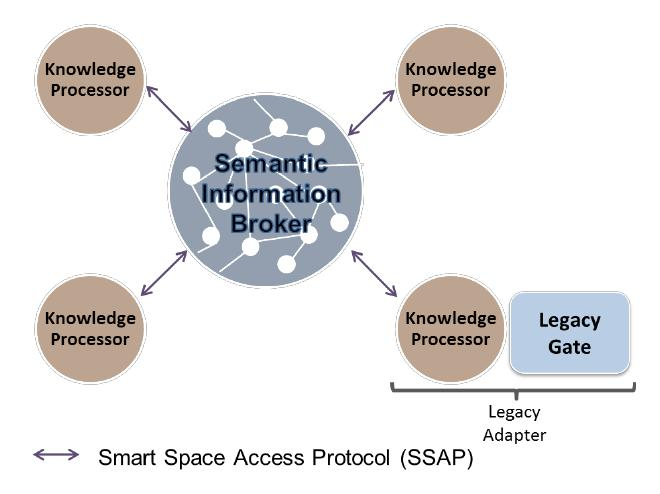
\includegraphics[width=0.5\textwidth]{assets/smart-m3.jpg}
	\caption{Architettura Smart-M3}
	\label{fig:smart-m3}
\end{figure}

\subsection{Le triple RDF}

Nell'architettura Smart-M3 le informazioni sono rappresentate in formato RDF (Resource Description Framework). In RDF le informazioni sono rappresentate come una tripletta \emph{soggetto, predicato, oggetto}. Le triple vengono memorizzate nel SIB e formano un grafo etichettato diretto il quale non necessariamente è un grafo connesso.

\subsection{Ontologie}

Mentre RDF fornisce il modello di dati standard per la rappresentazione delle informazioni, l'uso di un linguaggio ontologico è indispensabile per assegnare una semantica all'informazione. Linguaggi ontologici come RDFS e OWL forniscono un vocabolario comune. L'uso di una ontologia comune consente a tutti gli attori (uomini e macchine) di capire reciprocamente la semantica delle informazioni e di cooperare in simbiosi attraverso il SIB. Smart-M3 è agnostico rispetto all'ontologia e quindi consente agli sviluppatori di scegliere il modo migliore di modellare le informazioni al fine di soddisfare le esigenze funzionali del dominio applicativo indirizzato.

\subsection{Sottoscrizioni}

Un aspetto fondamentale di questa tecnologia è il meccanismo delle sottoscrizioni grazie al quale è possibile ricevere notifiche al variare di set di triple. Le sottoscrizioni sono determinanti nella nostra architettura perché, come vedremo più avanti (Sez. ~\ref{sec:protocol}), sono alla base dei protocolli di scambio dati tra i componenti del sistema.

\subsection{SPARQL}

SPARQL, si pronuncia sparkle, (acronimo ricorsivo di SPARQL Protocol and RDF Query Language) è il linguaggio standard de facto per interrogare dei dataset RDF. Come si può dedurre dal nome stesso SPARQL non è semplicemente un linguaggio di interrogazione di dati RDF, ma definisce anche il protocollo applicativo utilizzato per comunicare con le sorgenti RDF (si tratta di un binding su HTTP).

Così come SQL riflette, nella rappresentazione della query, il modello relazionale sottostante, allo stesso modo SPARQL basa la rappresentazione della query sul concetto di tripla e di grafo. Il meccanismo alla base della rappresentazione di una query e della ricerca della sua risposta è il graph matching. La query rappresenta un pattern di un grafo (RDF) e la risposta alla query sono tutte le triple (sotto-grafo) che fanno match con il pattern.

\subsection{Il protocollo SSAP}

L'SSAP (\emph{Smart Space Access Protocol}) è il protocollo con cui si comunica con il SIB (\cite{smart2010}). Il protocollo è session-based, i KP che vogliono comunicare con lo smart-space dovranno prima aderirvi con un operazione di Join prevista dall'SSAP. Il KP fornisce le sue credenziali nel messaggio di Join, il SIB esamina le credenziali e decide se accetare il KP o meno. Dopo l'operazione di Join, il KP può eseguire le altre operazioni. 
L'SSAP è il punto di integrazione principale dell'architettura Smart-M3. Le implementazioni di SIB e KP devono implementare tutte le operazioni del protocollo SSAP al fine di garantire l'interoperabilità.

Le operazioni supportate dal protocollo SSAP sono:

\begin{itemize}
	\item \textbf{JOIN}:
	\item \textbf{LEAVE}:
	\item \textbf{INSERT}:
	\item \textbf{REMOVE}:
	\item \textbf{UPDATE}:
	\item \textbf{QUERY}:
	\item \textbf{SUBSCRIBE}:
	\item \textbf{UNSUBSCRIBE}:
\end{itemize}
